\documentclass[12pt, oneside]{article}
\usepackage[letterpaper, margin=1in, headsep=0.5in, left=0.3in, right=2.5in]{geometry}
\usepackage[english]{babel}
\usepackage[utf8]{inputenc}
\usepackage{amsmath}
\usepackage{amsfonts}
\usepackage{amssymb}
\usepackage{tikz}
\usepackage{yhmath}
\usetikzlibrary{quotes, angles}
\usepackage{graphicx}
\usepackage{enumitem}
\usepackage{multicol}

\newif\ifmeta
\metatrue %print standards and topics tags

\title{Regents Geometry}
\author{Chris Huson}
\date{May 2022}

\usepackage{fancyhdr}
\pagestyle{fancy}
\fancyhf{}
\renewcommand{\headrulewidth}{0pt} % disable the underline of the header
\raggedbottom

%\fancyhead[LE]{\thepage}
\fancyhead[RO]{Name:}
\fancyhead[LO]{BECA / Dr. Huson / Geometry Regents Mixed Review}
\cfoot{\thepage}

\begin{document}
\subsubsection*{11.16 Transversal similarity}
\begin{enumerate}[itemsep=1.1cm]
\item In the diagram below, $\overline{AF}$ and $\overline{DB}$ intersect at $C$, and $\overline{AD}$ and $\overline{FBE}$ are drawn such that $\textup{m}\angle D = 70^\circ$, $\textup{m}\angle CBE = 110^\circ$, $DC=9.2$, $AC=11.2$, and $FC=25.2$.
  \begin{center}
  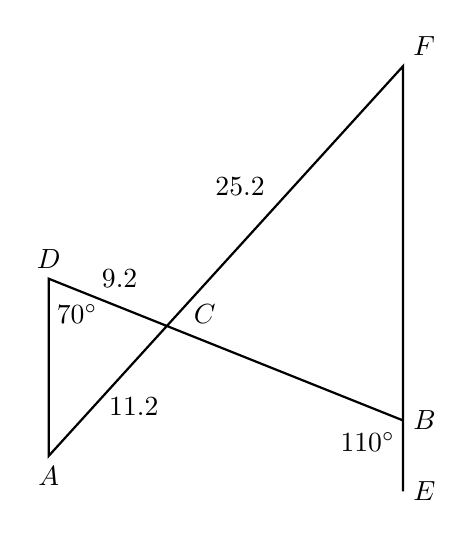
\begin{tikzpicture}[scale=0.9]
    \draw [thick]
      (0,0)node[right]{$B$}--
      (-5,2)node[above]{$D$}--
      (-5,-0.5)node[below]{$A$}--
      (0,5)node[above right]{$F$}--
      (0,-1)node[right]{$E$};
      \node at (-2.8,1.5){$C$};
      \node at (-0.5, -0.3){$110^\circ$};
      \node at (-4.6, 1.5){$70^\circ$};
      \node at (-4, 2){$9.2$};
      \node at (-3.8, 0.2){$11.2$};
      \node at (-2.3, 3.3){$25.2$};
  \end{tikzpicture}
  \end{center}
  What is the length of $\overline{CB}$?

\item The line represented by $3y=2x+9$ is dilated by a scale factor of $k$ centered at the origin, such that the image of the line has an equation of $y= - \frac{2}{3}x+6$. What is the scale factor?

\item A rectangular tabletop will be made of solid oak that weighs 47 pounds per cubic foot. The tabletop will have a length of six feet, a width of two and a half feet, and a thickness of two inches. Determine and state the weight of the tabletop, in pounds.

\item The equation of a cirle is $x^2+y^2-8x+2y=8$. What are the center and radius of the circle?

\item Directed line segment $DE$ has endpoints $D(3, 7)$ and $E(3,-2)$. Point $P$ divides such that $DP:PE$ is $1:2$. What are the coordinates of $P$?

\newpage
\item In the diagram below of $\triangle ROC$ and $\triangle MUS$, angles $C$ and $S$ are right angles, and $\triangle ROC \sim \triangle MUS$
\begin{center}
  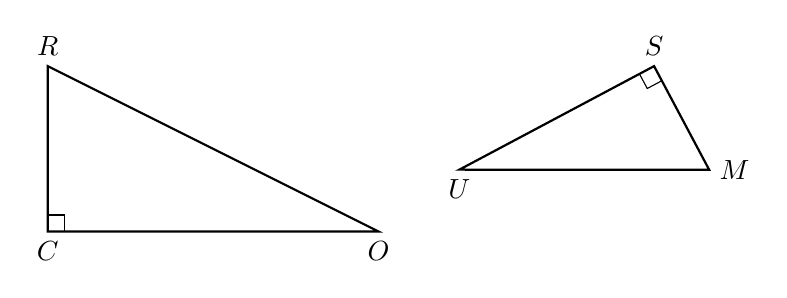
\begin{tikzpicture}[scale=0.7]
  \draw [thick, xshift=4cm, yshift=2cm, rotate=208]
    (0,0)node[above]{$S$}--
    (4,0)node[below]{$U$}--
    (0,2.13)node[right]{$M$}--cycle;
    \draw [xshift=4cm, yshift=2cm, rotate=208]
      (0,0)++(0.3,0)--++(0,0.3)--+(-0.3,0);
  \draw [thick]
    (-1,-1)node[below]{$O$}--
    (-7,2)node[above]{$R$}--
    (-7,-1)node[below]{$C$}--cycle;
    \draw (-7,-1)++(0.3,0)--++(0,0.3)--+(-0.3,0);
\end{tikzpicture}
\end{center}
If $RO=17$ and $RC=7.5$, what is the measure of $\angle U$, to the \emph{nearest degree}?

\item Directed line segment $DE$ has endpoints $D(-4, -2)$ and $E(1,8)$. Point $F$ divides such that $DF:FE$ is $2:3$. What are the coordinates of $F$?

\item If an right triangle is continuously rotated around one of its legs, which 3-dimensional object is generated?
    \begin{enumerate}
      \item cone
      \item sphere
      \item pyramid
      \item prism
    \end{enumerate}

\item In diagram below of right triangle $ABC$, altitude $\overline{BD}$ is drawn.
  \begin{center}
    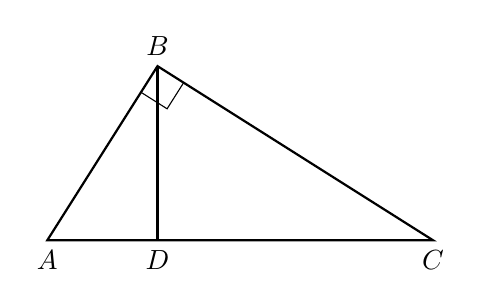
\begin{tikzpicture}[scale=0.7]
    \draw [thick]
    (0,0)node[below]{$A$}--
    (7,0)node[below]{$C$}--
    (2,3.16)node[above]{$B$}--cycle;
    \draw (2,3.16)++(-0.15*2,-0.15*3.16)--++(0.15*3.16,-0.15*2)--+(0.15*2,0.15*3.16);
    \draw [thick](2,0)node[below]{$D$}--(2,3.16);
  \end{tikzpicture}
  \end{center}
    Which ratio is always equivalent to $\sin A$?
    \begin{multicols}{2}
    \begin{enumerate}
        \item $\displaystyle \frac{AB}{BD}$
        \item $\displaystyle \frac{BD}{BC}$ 
        \item $\displaystyle \frac{CD}{BC}$
        \item $\displaystyle \frac{BC}{AB}$
    \end{enumerate}
    \end{multicols}

\end{enumerate}
\end{document}
  